\documentclass[twoside]{article}
\usepackage{graphics}
\usepackage{graphicx}
\usepackage{titlesec}
\setlength{\oddsidemargin}{0.25 in}
\setlength{\evensidemargin}{-0.25 in}
\setlength{\topmargin}{-0.6 in}
\setlength{\textwidth}{6.5 in}
\setlength{\textheight}{8.5 in}
\setlength{\headsep}{0.75 in}
\setlength{\parindent}{0 in}
\setlength{\parskip}{0.1 in}

%
% The following commands set up the lecnum (lecture number)
% counter and make various numbering schemes work relative
% to the lecture number.
%
\newcounter{lecnum}
\renewcommand{\thepage}{\thelecnum-\arabic{page}}
\renewcommand{\thesection}{\thelecnum.\arabic{section}}
\renewcommand{\theequation}{\thelecnum.\arabic{equation}}
\renewcommand{\thefigure}{\thelecnum.\arabic{figure}}
\renewcommand{\thetable}{\thelecnum.\arabic{table}}

%
% The following macro is used to generate the header.
%
\newcommand{\lecture}[4]{
   \pagestyle{myheadings}
   \thispagestyle{plain}
   \newpage
   \setcounter{lecnum}{#1}
   \setcounter{page}{1}
   \noindent
   \begin{center}
   \framebox{
      \vbox{\vspace{2mm}
    \hbox to 6.28in { {\bf EE 382V: Social Computing
                        \hfill Fall 2018} }
       \vspace{4mm}
       \hbox to 6.28in { {\Large \hfill Lecture #1, Session 4: #2  \hfill} }
       \vspace{2mm}
       \hbox to 6.28in { {\it Lecturer: #3 \hfill Scribe: #4} }
      \vspace{2mm}}
   }
   \end{center}
   \markboth{Lecture #1: #2}{Lecture #1: #2}
   %{\bf Disclaimer}: {\it These notes have not been subjected to the
   %usual scrutiny reserved for formal publications.  They may be distributed
   %outside this class only with the permission of the Instructor.}
   \vspace*{4mm}
}

%
% Convention for citations is authors' initials followed by the year.
% For example, to cite a paper by Leighton and Maggs you would type
% \cite{LM89}, and to cite a paper by Strassen you would type \cite{S69}.
% (To avoid bibliography problems, for now we redefine the \cite command.)
% Also commands that create a suitable format for the reference list.
\renewcommand{\cite}[1]{[#1]}
\def\beginrefs{\begin{list}%
        {[\arabic{equation}]}{\usecounter{equation}
         \setlength{\leftmargin}{2.0truecm}\setlength{\labelsep}{0.4truecm}%
         \setlength{\labelwidth}{1.6truecm}}}
\def\endrefs{\end{list}}
\def\bibentry#1{\item[\hbox{[#1]}]}

%Use this command for a figure; it puts a figure in wherever you want it.
%usage: \fig{NUMBER}{SPACE-IN-INCHES}{CAPTION}
\newcommand{\fig}[3]{
			\vspace{#2}
			\begin{center}
			Figure \thelecnum.#1:~#3
			\end{center}
	}
% Use these for theorems, lemmas, proofs, etc.
\newtheorem{theorem}{Theorem}[lecnum]
\newtheorem{lemma}[theorem]{Lemma}
\newtheorem{proposition}[theorem]{Proposition}
\newtheorem{claim}[theorem]{Claim}
\newtheorem{corollary}[theorem]{Corollary}
\newtheorem{definition}[theorem]{Definition}
\newenvironment{proof}{{\bf Proof:}}{\hfill\rule{2mm}{2mm}}

% **** IF YOU WANT TO DEFINE ADDITIONAL MACROS FOR YOURSELF, PUT THEM HERE:

\begin{document}



%\lecture{**LECTURE-NUMBER**}{**DATE**}{**LECTURER**}{**SCRIBE**}
\lecture{4}{September 29}{Vijay Garg}{Zeid Ayssa}

\section{Stable Marriage Optimality}



After we introduced $Gale-Shapley$ stable matching algorithm, we need to prove that the resulting matching is optimal i.e. there is no better matching for men.

\textbf{Note:} throughout this section, we will assume men optimal matching. Furthermore, lower ranking numbers mean higher preference i.e.$1$ means it is the man's/woman's $1^{st}$ choice and $4$ means that it is the man's/woman's $4^{th}$ choice.

Assuming men optimal assignment, Below is the Hasse diagram of all possible assignments. Note that this is not necessarily matching assignments, but rather all possible men assignments to women. This is not necessarily a matching due to the fact that if all men were matched to their first woman preference, we could have multiple men preferring the same women and we cannot match a women to more than one man.

\begin{figure}[htp]
\centering
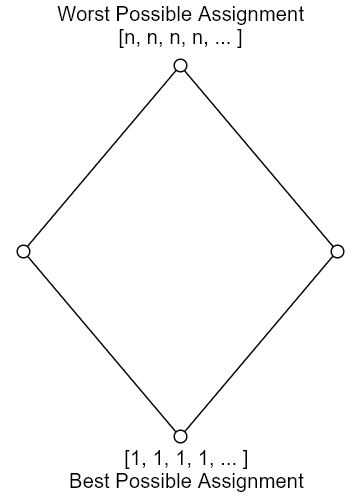
\includegraphics[width=5cm]{Hasse_Diagram_All_Possible_Assigments.JPG}
\caption{Hasse diagram of all possible men assignments}
\label{fig:allPossibleMenAssigments}
\end{figure}

\textbf{Example:} if we have two matchings $M_1 = [1, 2, 1, 3, 1]$ and $M_2 = [2, 3, 2, 3, 1]$, if $M_1 \leq M_2$, where $M_1 \leq M_2$ is defined as $ \forall i:  M_1[i] \leq M_2[i]$, then we know that every man in $M_1$ is either happier or as happy compared to $M_2$ matching.

Let $u$ and $v$ be vectors of size $n$ representing two different men assignments in figure~\ref{fig:allPossibleMenAssigments} where $u \leq v$ is defined as $ \forall i:  u[i] \leq v[i]$

We know from a previous section that figure~\ref{fig:allPossibleMenAssigments} is a Partially Ordered Set (POSET) because it is Reflexive, Anti-Symmetric, and Transitive.

\begin{claim}{$(X, \leq$) is a lattice poset where $X$ is the set of all possible assignments shown in figure~\ref{fig:allPossibleMenAssigments}}
\end{claim}

\begin{definition}{A poset is lattice if every two elements in the poset have a unique upper bound or join and a unique lower bound or meet. Minimum upper bound or join is denoted by $\sqcup$ and maximum lower bound or meet is denoted by $\sqcap$.}
\end{definition}

\begin{figure}[htp]
\centering
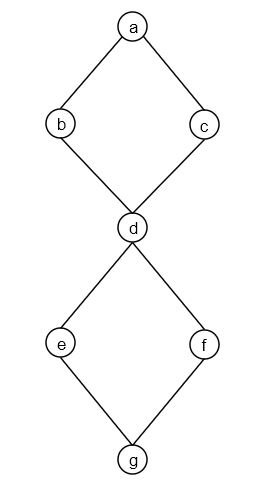
\includegraphics[width=5cm]{Hasse_Diagram_Lattice_Example.JPG}
\caption{Hasse diagram of a lattice poset}
\label{fig:latticeExample}
\end{figure}

Figure~\ref{fig:latticeExample} is an example of a lattice poset i.e. for every two elements there is a unique upper and lower bounds. Let us check:

$b \sqcap c = d$ and $b \sqcup c = a$

$e \sqcap c = g$ and $e \sqcup c = a$

\begin{proof} Let $u$ and $v$ be two different assignment sets with size $4$

$u[1, 3, 2, 1]$

$v[2, 1, 3, 1]$

$w = u \sqcap v = [1, 1, 2, 1]$ i.e. pairwise min operation.

We know that $w \leq u$ and $w \leq v$, so $w$ is a more preferable matching to men than $u$ or $v$. This also means that $w$ will always be greater than or equal to any other assignment set that is less than or equal to $u$ or $v$. For example, if there is another set $g = [1, 1, 1, 1]$ then $g < u$ and $g < v$ $\Longrightarrow g \neq w \Longrightarrow w > g$ since $w$ is already defined as the meet between sets $u$ and $v$. This proves that the poset is a lattice poset.
\end{proof}

\begin{claim}{$(X, \leq$) is a distributed lattice poset}
\end{claim}

We need to verify that poset $(X\leq)$ is a distributive lattice.

Let $x = [a_1, a_2, a_3, \ldots]$, $y = [b_1, b_2, b_3, \ldots]$, and $z = [c_1, c_2, c_3, \ldots]$ be different sets in the poset. For a poset to be a distributed lattice we need to verify that $a \sqcap (b \sqcup c) = (a \sqcap b) \sqcup (a \sqcap c)$ which means we need to verify that:

$min(a_x, max(b_x,c_x) = max (min(a_x,b_x), min(a_x,c_x))$

\begin{proof} Let $x[1, 3, 2, 1]$, $y[2, 2, 3, 1]$, and $z[3, 1, 2, 3]$ be three different assignment sets with size $4$. Now, let us see if this is a distributed lattice. 

\underline{$1^{st} Element$}

$min(1, max(2, 3)) = min(1, 3) = 1$

$max(min(1, 2), min(1, 3)) = max(1, 1) = 1$

\underline{$2^{nd} Element$}

$min(3, max(2, 1)) = min(3, 2) = 2$

$max(min(3, 2), min(3, 1)) = max(2, 1) = 2$

\underline{$3^{rd} Element$}

$min(2, max(3, 2)) = min(2, 3) = 2$

$max(min(2, 3), min(2, 2)) = max(2, 2) = 2$

\underline{$4^{th} Element$}

$min(1, max(1, 3)) = min(1, 3) = 1$

$max(min(1, 1), min(1, 3)) = max(1, 1) = 1$

Given that for all elements in the assignment sets $x$, $y$, and $z$ the result of $min(a_x, max(b_x,c_x)$ was equal to the result of $max (min(a_x,b_x), min(a_x,c_x))$, then this is a distributive assignment set. Since this should hold true for all possible assignment sets in our poset $(X, \leq)$ then we can say that this is a distributed lattice.\end{proof}

Why do we care if it is a distributed lattice or not? If a poset is a distributive lattice then it makes it similar to Boolean algebra since union and intersection distribute over each other. This property will allow us define a Boolean predicate later on to help us prove optimal stable matching.

\subsection{Hasse Diagram of All Assignments and Stable Matching Region}

\begin{figure}[htp]
\centering
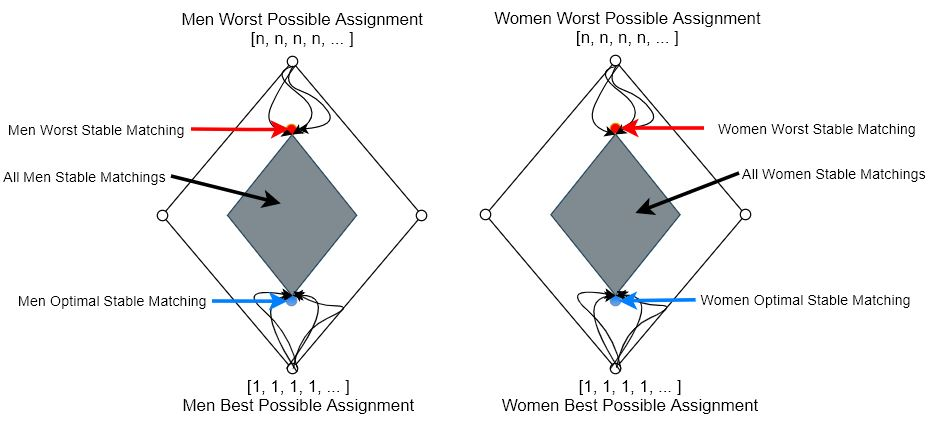
\includegraphics[width=13cm]{Hasse_Diagram_All_Possible_Stable_Matching.JPG}
\caption{Hasse diagram of all possible assignments along with the stable matching region}
\label{fig:allPossibleStableMatchings}
\end{figure}

Figure~\ref{fig:allPossibleStableMatchings} shows the Hasse diagram of all possible assignments. It also shows the men optimal and women optimal stable matching. There is a region that has different sets of stable matching i.e. no blocking pair, but there is only one optimal stable matching for men and women. 

A men optimal stable matching is a matching where there is no other stable matching set that leads to happier men i.e. there is no other stable set that is less than the current stable matching. The same applies to women where a women optimal stable matching is a matching where there is no other stable matching set that leads to happier women i.e. there is no other stable set that is less than the current stable matching.

Starting from the initial set $[1, 1, 1, \ldots]$ and taking any path when using $Gale-Shapley$ algorithm will always give us the optimal men or women stable matching.

\subsection{Finding Stable Matching Assignments}

If we want to write an algorithm to find the optimal stable matching, we need to figure out some sort of logic to determine if the current man and woman matching is the best we can do before moving on. Trying to go over all the possible matchings would take a lot of time since the total number of possible assignments is $n^n$ because for every man there are n women i.e. $ m = [ \ldots n] \Longrightarrow [n][n]$ array.

\begin{figure}[htp]
\centering
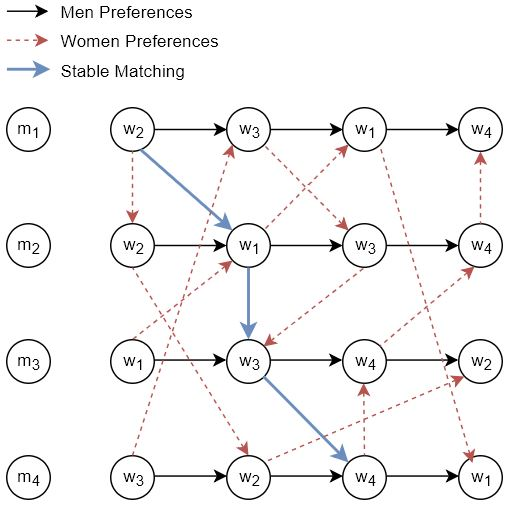
\includegraphics[width=9cm]{PossibleStableMatchings.JPG}
\caption{Possible men and women matching}
\label{fig:PossibleStableMatchings}
\end{figure}

Figure~\ref{fig:PossibleStableMatchings} shows the preference for men and women where we can formally represent them as:

\underline{Men Preferences:}

$m_1 = [2, 3, 1, 4]$

$m_2 = [2, 1, 3, 4]$

$m_3 = [1, 3, 4, 2]$

$m_4 = [3, 2, 4, 1]$

\underline{Women Preferences:}

$w_1 = [3, 2, 1, 4]$

$w_2 = [1, 2, 4, 3]$

$w_3 = [4, 1, 2, 3]$

$w_4 = [4, 3, 2, 1]$

Figure~\ref{fig:PossibleStableMatchings} also shows one possible stable matching $\{\{m_1, w_2\}, \{m_2, w_1\}, \{m_3, w_3\}, \{m_4, w_4\}\}$.

\subsubsection{Forbidden State}

Figure~\ref{fig:forbiddenState} shows a matching that has a forbidden state. We can see from figure~\ref{fig:forbiddenState} that $w$ prefers $m'$ more than $m$, we can also see that $m'$ prefers $w$ more than $w'$, therefore this a blocking pair which means that this is not a stable matching.

From figure~\ref{fig:forbiddenState} we can say that a matching is not stable if there is a preference arrow that points to a node before the current matching region since it will represent a blocking pair. Similarly, we can say that a matching is stable if there are no preference arrows pointing to a node that is before the current matching region. If our algorithm makes sure that there are no forbidden states, then we know for sure that if a women rejects a man then there is no way there was going to be a stable marriage that would include this pair. If a matching does not include a forbidden state, then this also proves the claim that this is a distributed lattice.

\begin{figure}[htp]
\centering
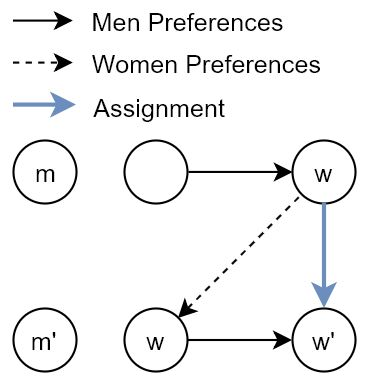
\includegraphics[width=5cm]{ForbiddenStateExample.JPG}
\caption{Forbidden state}
\label{fig:forbiddenState}
\end{figure}

Figure~\ref{fig:PossibleStableMatchingsWithForbiddenMatching} shows a matching that has a blocking pair or a forbidden state. A matching with a forbidden state means that the matching is not stable.

\begin{figure}[htp]
\centering
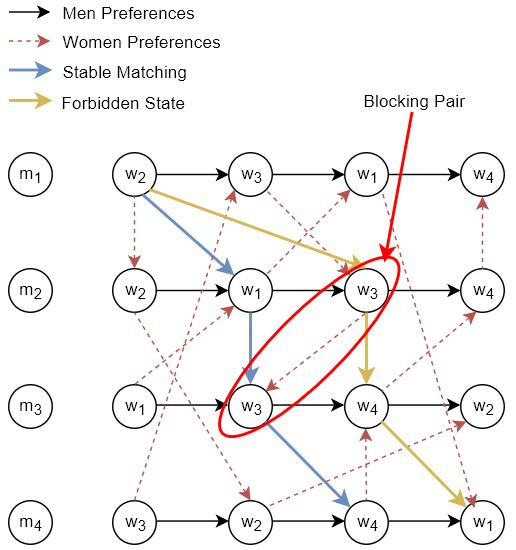
\includegraphics[width=9cm]{PossibleStableMatchingsWithForbiddenMatching.JPG}
\caption{Possible men and women matching}
\label{fig:PossibleStableMatchingsWithForbiddenMatching}
\end{figure}


\vspace*{1cm}In the next class we will go over a formal definition of the forbidden state and how it will help us prove that $Gale-Shapley$ algorithm will give us an optimal stable matching. We will define an algorithm that uses $(G, i, B)$ where:

$G:$ Assignment

$i:$ men

$B:$ Boolean Predicate, where $B$: 
\begin{itemize}
\item Is a matching 
\item Has no blocking pair
\end{itemize}

\end{document}






